\documentclass{article}
\usepackage[T1]{fontenc}
\usepackage{lmodern}
\usepackage{graphicx}
\usepackage{amsmath,amssymb}
\usepackage[a4paper,margin=2cm]{geometry}
\usepackage[absolute,overlay]{textpos}
\setlength{\TPHorizModule}{1mm}
\setlength{\TPVertModule}{1mm}
\usepackage[indonesian]{babel}
\usepackage{hyperref}
\setlength{\emergencystretch}{2em}
% unit: Halaman 56

\begin{document}

% === Halaman 56 (llm) ===

\vspace{160.68mm}

\begin{itemize}
  \item Pada Abad ke-17, sejarah kriptografi pernah mencatat korban di Inggris.
  \item Queen Mary of Scotland, dipancung setelah pesan rahasianya dari balik penjara (sebuah cipherteks yang isinya rencana membunuh Ratu Elizabeth I) pada Abad Pertengahan berhasil dipecahkan oleh Thomas Phelippes, seorang pemecah kode (codebreaker).
\end{itemize}

% deskripsi: Potret Queen Mary of Scotland
% bbox normalisasi: [0.6660, 0.2020, 0.9120, 0.7430]
\begin{textblock*}{51.66mm}(139.86mm,59.99mm)
\noindent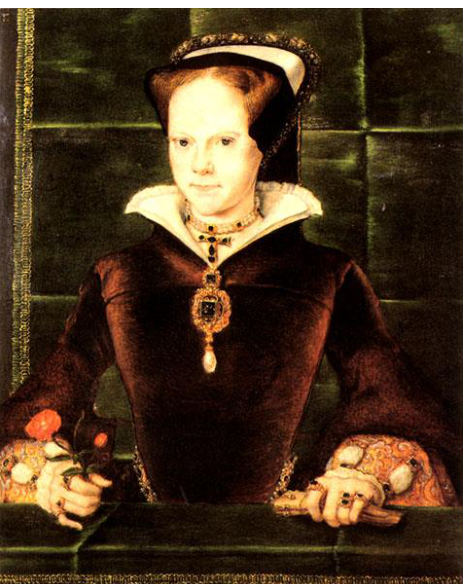
\includegraphics[width=51.66mm,height=160.68mm]{../../images/llm/page_056_img_01.png}%
\end{textblock*}

\end{document}
